\section*{Methods}
\label{Methods}
%
The psychometric method used for stimuli presentation is not one of the classical methods but is one of the adaptive methods, namely \textit{Transformed Up/Down Method}. Instead of pre-chosen stimuli intensities the stimuli intensities are determined by previous response and thus dose not depend on a qualified guess on where the threshold might be, same goes for other adaptive methods. By using an adaptive method the efficiency is maximizes because the stimuli presentations converges upon threshold and have fewer stimuli presentations faraway from threshold, \parencite[p. 287]{PDF:Hearing}.

There are different strategies on how to determine the needed step size e.g. It can be fixed or change as the presentations converges upon the threshold, \parencite[p. 22]{PDF:Psychoacoustic}. In this study it is decided to use a changing step size, the steps will change in a logarithmic manner so that the steps are either halved or doubled according to the previous response. Apart from higher efficiency \textit{Transformed Up/Down Method} yield higher accuracy compared to e.g. \textit{Method of Constant Stimuli} because the step size is altered according to previous response. Furthermore \textit{Transformed Up/Down Method} follow the test subject's response criterions so it always adjusts the stimuli intensities according to the previous answers.  

The specific up/down rules are chosen so that the stimuli intensities will converge around threshold read as close to 75 \%, on a psychometric function, as possible. To achieve this the up/down rules are defined as one-up and two-down, which will result in a threshold read at 70.7 \%, \parencite[p. 22]{PDF:Psychoacoustic}. This rule implies that one-up is a result of an incorrect answer, which will lead to an increase in stimulus intensity and two-down is a result of two consecutive correct answers, which will lead to a decrease in stimulus intensity. According to \textcite[p. 293]{PDF:Hearing}, the probability of an increasing stimulus intensity due to an incorrect answer is: 
%
\begin{equation}
	(1-p)+p\cdot(1-p)
\end{equation}  
%
And for a decreasing stimulus intensity due to two consecutive correct answers: 
%
\begin{equation}
	p\cdot p = p^2
\end{equation}    
%       
According to \textcite[p. 293]{PDF:Hearing} the chosen strategy will converge on a point where both rules have the same probability, which is 0.5. For a decreasing stimulus intensity the probability is therefore:
%
\begin{equation}
	p^2=0.5
\end{equation}  
%
And the probability for a single correct answer is: 
%
\begin{equation}
	p = \sqrt{p^2} \Rightarrow p = \sqrt{0.5} = 0.707
\end{equation}
%
So the probability for a single correct answer is 70.7 \%. On \autoref{fig:IllustrationUpDown} an illustration of the psychometric function for a \textit{Transformed 1-Up/2-Down Method} is presented. 
%
\begin{figure}[H]
	\centering
	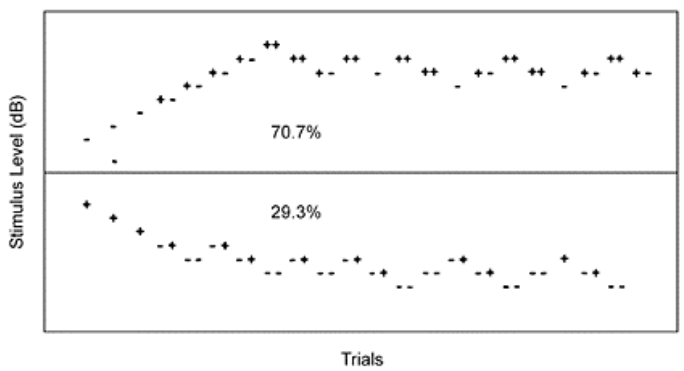
\includegraphics[resolution=300,width=0.7\textwidth]{Figure/IllustrationOfUpDown}
	\caption{An illustration of how the stimuli intensities converges upon threshold at 70.7 \% (upper frame) and 29.3 \% (lower frame), \parencite[p. 294]{PDF:Hearing}. In the upper frame the minuses indicates an incorrect answer and the pluses indicate a correct answer, and vice versa in the lower frame.}
	\label{fig:IllustrationUpDown}
\end{figure}
\noindent
%
The threshold is calculated by averaging the stimuli intensity level at the last four or six reversals, this will be determined based on results from a pilot test. A reversal is defined as when the stimulus intensity changes direaction from either a decreasing intensity, due to two consecutive correct answers, or a increasing intensity, due to one incorrect answer. A stop criterion for the test is determined, the criterion is set at eight reversals (KILDE?). The number of trials needed to find the threshold with  \textit{Transformed 1-Up/2-Down Method} must be less than the 100 trials used in \textit{Method of Constant Stimuli}, because it is assumed that \textit{Transformed 1-Up/2-Down Method} is more efficient and accurate than \textit{Method of Constant Stimuli}. Therefore, a maximum of 100 trials is defined as a stop criterion if, against our assumption, the threshold is not reach within eight reversals. The first trial consist of a reference 800 Hz tone and a comparison 876.8 Hz tone, the comparison tone changes in aforementioned logarithmic steps. After two consecutive correct answers the comparison would be made between 800 Hz and 838.4 Hz.

Because one of the goals for this study is to do a comparison of the results achieved by a \textit{Transformed 1-Up/2-Down Method} and from the \textit{Method of Constant Stimuli}, it is an advantage to present the same stimuli intensities in both methods, which is why the first comparison tone is 876.8 Hz. Both reference and comparison tone have a duration of 1 second.\blankline
%               
Data collections is done by \textit{Two-Alternative Forced Choice}, 2-AFC, which is possible because threshold converges on the 70.7 \% point and not the 50 \% point as with a \textit{Simple Up/Down Method}. A more objective measure is obtained with 2-AFC because the test subjects are forced to make an answer whether or not they actually heard a difference between the two stimuli, \parencite[p. 1219]{PDF:PsyphyMethods}.\blankline 
%
Both \textit{Transformed 1-Up/2-Down Method} and \textit{Simple Up/Down Method} yields higher efficiency and accuracy compared to e.g. \textit{Method of Constant Stimuli}, furthermore both of the adaptive methods changes according to the test subject's answer criterions, which \textit{Method of Constant Stimuli} does not. One problem with \textit{Simple Up/Down Method} is, that it is transparent so the test subjects easily can predict how the stimuli are presented and answer accordingly. In addition it is not advised to use 2-AFC with a \textit{Simple Up/Down Method} because it already converges on the 50 \% point, which is also the guessing probability for 2-AFC, this is avoided with a \textit{Transformed 1-Up/2-Down Method}. Furthermore \textit{Transformed 1-Up/2-Down Method} requires two consecutive correct answers before the intensity decreases, this will expose if the test subject is merely guessing which of the of two stimuli had the highest pitch. 

On the other hand, one of the disadvantages with \textit{Transformed 1-Up/2-Down Method} is that it collects more non-informative answers compared to \textit{Simple Up/Down Method}. This is due to the used up and down rules, there needs to be two consecutive correct answers before a decreasing intensity is obtained, which in turns makes the \textit{Transformed 1-Up/2-Down Method} a bit less efficient compared to the \textit{Simple Up/Down Method}. A general disadvantages with \textit{Transformed Up/Down Method} is that not all points on the psychometric function can be reached.          
%